\addcontentsline{toc}{section}{Introduction}
\section*{Introduction}

Dans ce chapitre, nous explorerons la schématisation détaillée du projet visant à remplacer notre architecture monolithique par une approche basée sur des microservices et des micro-frontends, tout en migrer notre système de gestion de base de données de MariaDB vers Delta Lake. Cette transition marque une étape cruciale dans notre parcours d'évolution technologique, offrant des avantages significatifs en termes de flexibilité, d'évolutivité et de maintenabilité.

\section{Schématisation}

Dans le cadre de la schématisation de la solution, nous avons opté pour une architecture basée sur des microservices, utilisant les technologies suivantes : Spring Data, JPA, Hibernate, JDBC et Trino.

Les microservices sont développés en utilisant Spring Data, qui fournit une abstraction de haut niveau pour interagir avec la base de données. Cela permet d'utiliser des annotations et des interfaces pour définir les entités, les requêtes et les opérations de persistance. JPA (Java Persistence API) est utilisé comme couche d'interface pour interagir avec la base de données, tandis que Hibernate est utilisé comme fournisseur de persistance, permettant la gestion des objets Java et leur mapping vers Trino.

La communication entre les microservices est assurée par un broker Kafka. Kafka est une plateforme de streaming distribuée qui permet aux microservices d'échanger des messages en temps réel. Les microservices publient des événements sur des sujets Kafka, et d'autres microservices peuvent s'abonner à ces sujets pour recevoir les événements correspondants.

Pour gérer l'authentification et l'autorisation, nous utilisons Spring Cloud Gateway. Ce composant reçoit les appels de services provenant des applications Web, mobiles ou de bureau. Ces applications envoient un jeton JWT (JSON Web Token) à Spring Cloud Gateway pour authentification. Ce dernier vérifie la disponibilité du jeton en contactant Keycloak, qui est responsable de la gestion des identités et des accès. Une fois le jeton validé, Spring Cloud Gateway autorise la demande à passer vers les microservices.

Les microservices communiquent avec Trino en utilisant le connecteur JDBC\@. Trino est responsable de l'interrogation et du traitement des données sur une grande quantité de sources de données. Il stocke les métadonnées dans Hive, qui est un entrepôt de données basé sur Hadoop. Trino utilise également le concept de tables Delta pour gérer les modifications incrémentielles des données. Ces tables Delta sont stockées sur AWS (Amazon Web Services), offrant une solution de stockage évolutive et fiable.

\begin{figure}[H]
\centering
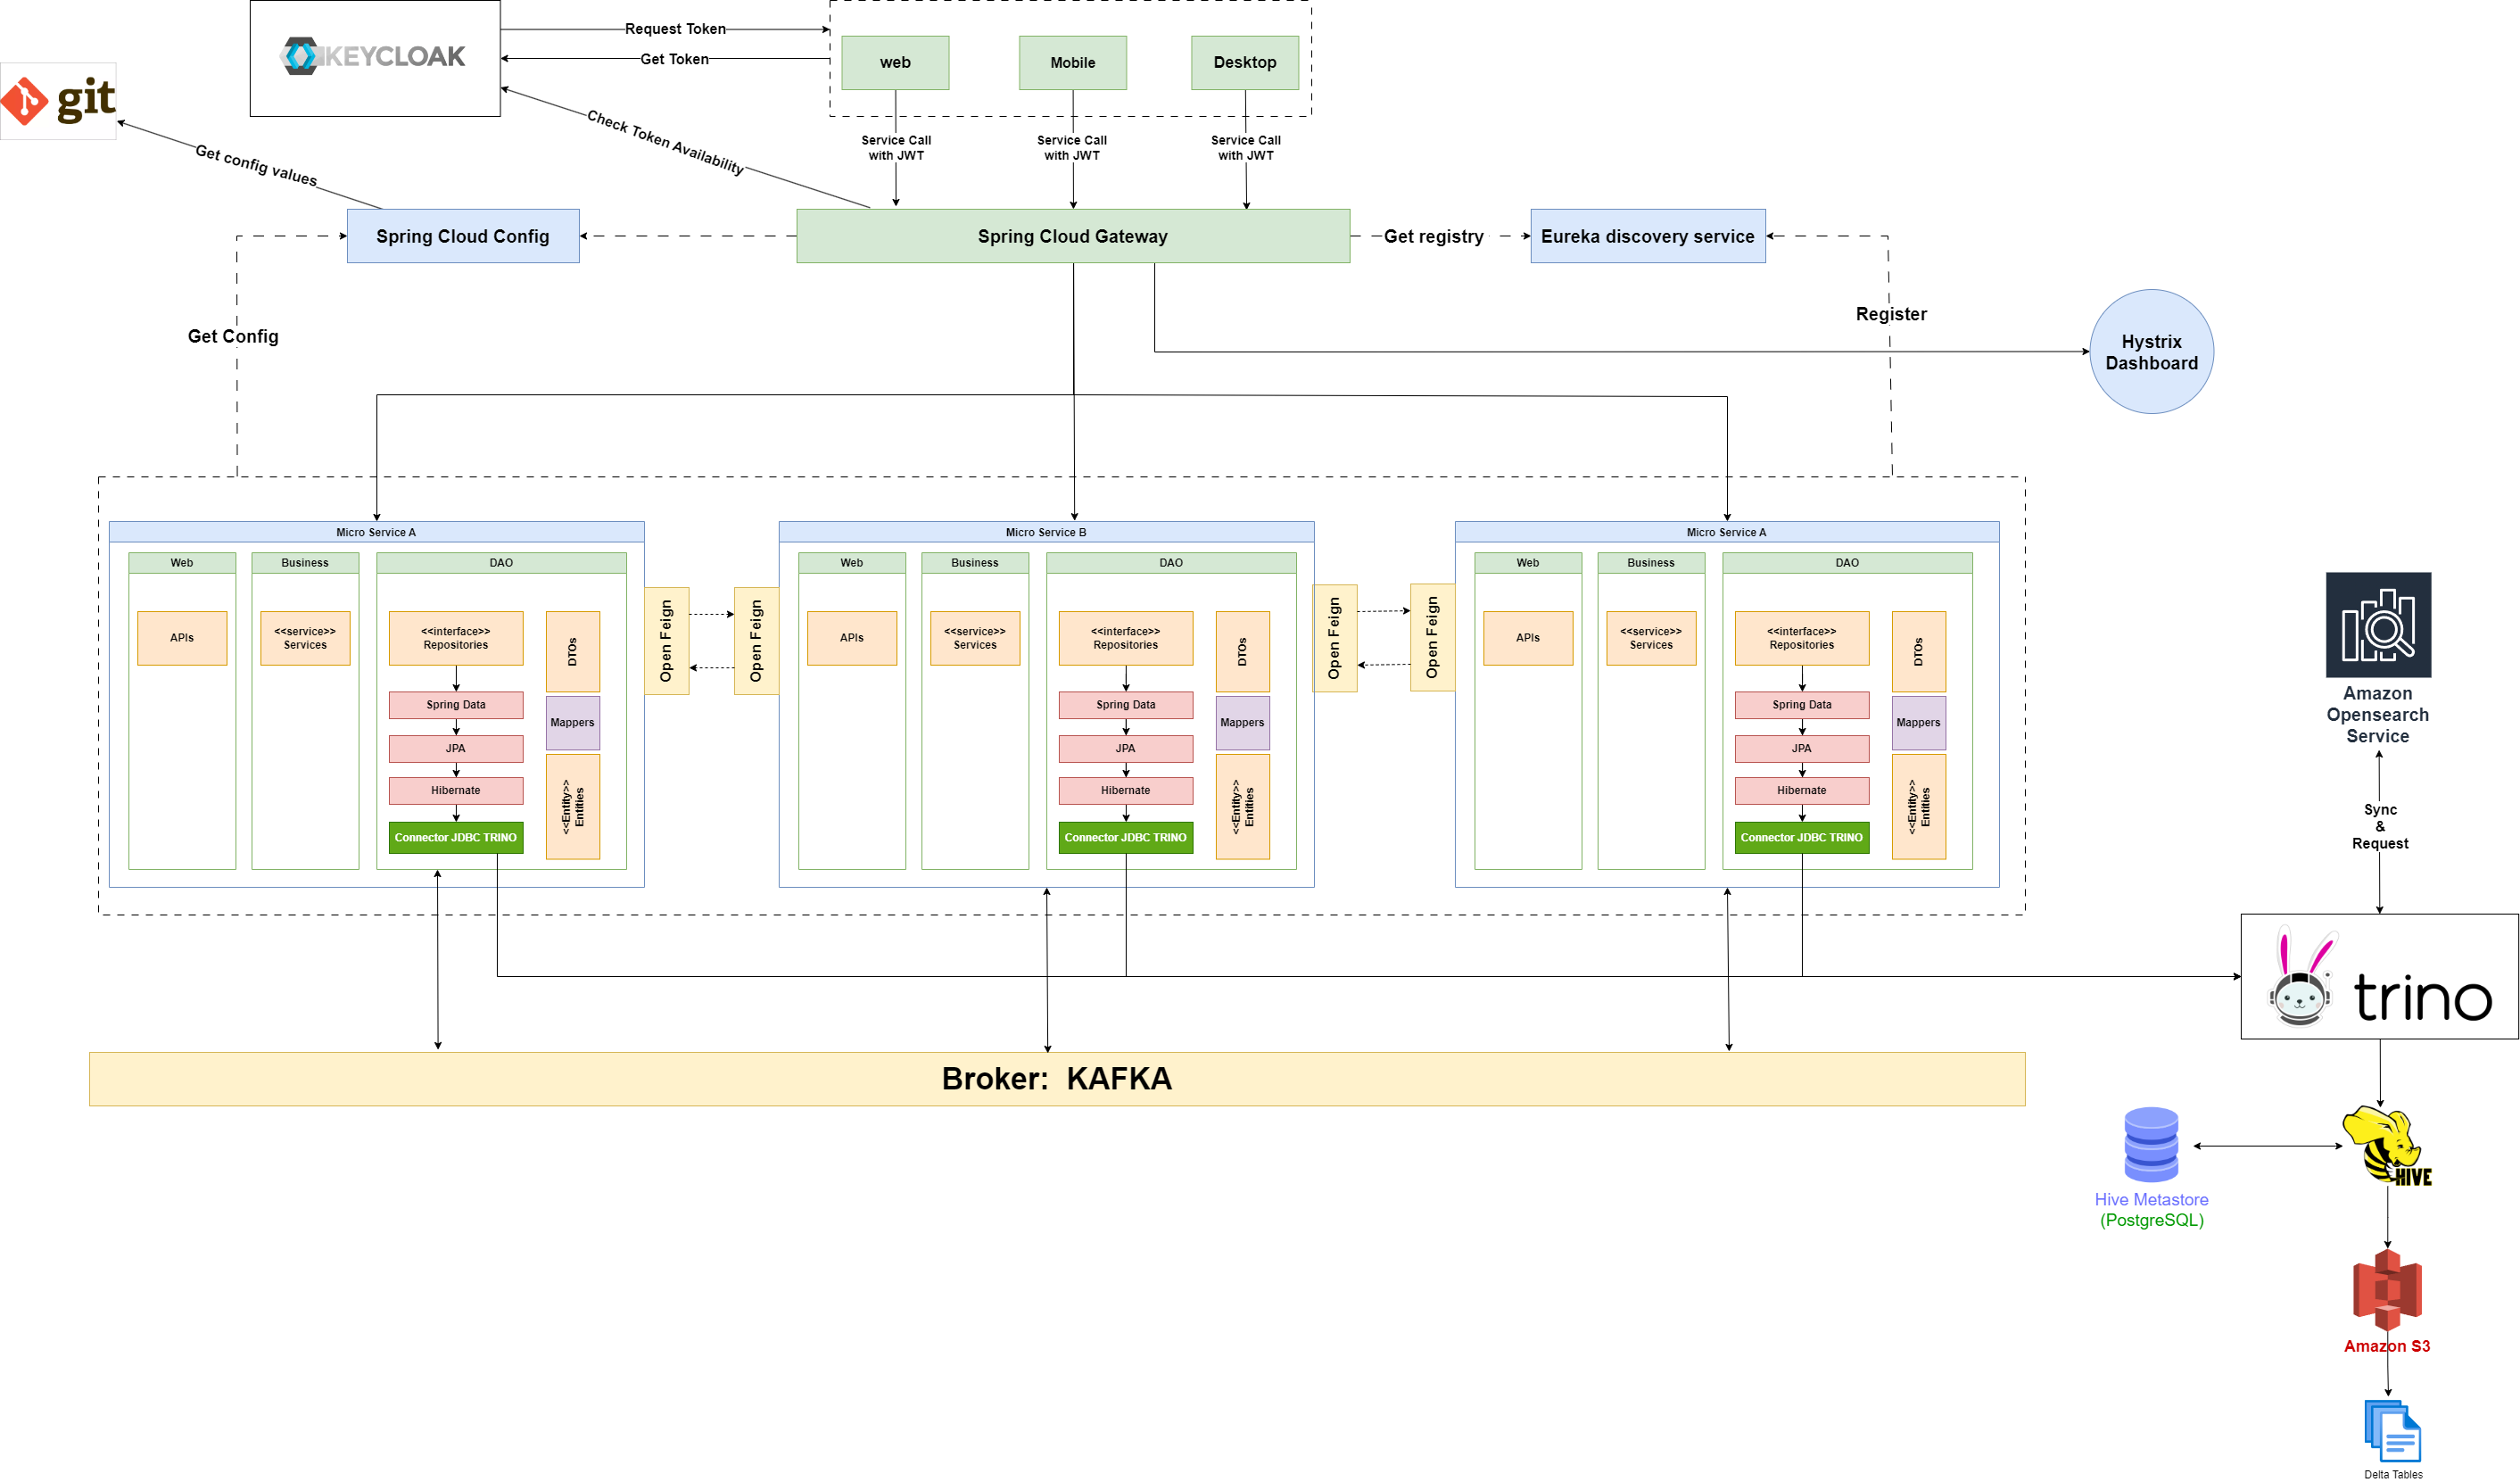
\includegraphics[width=\linewidth]{images/architecture-solution.png}
\caption{Architecture de solution}\label{fig:solution}
\end{figure}

\section{Avantages}

L'architecture que nous avons choisie présente plusieurs avantages significatifs :

\begin{enumerate}
    \item[$\bullet$] \textbf{Évolutivité:} L'architecture basée sur des microservices permet une évolutivité horizontale, ce qui signifie que chaque microservice peut être déployé et mis à l'échelle indépendamment en fonction de ses besoins spécifiques. Cela permet d'ajuster la capacité et les ressources de manière granulaire, ce qui facilite la gestion des charges de travail élevées et l'adaptation aux besoins croissants de l'application.
    \item[$\bullet$] \textbf{Modularité:} La conception modulaire des microservices permet une gestion plus efficace du développement, du déploiement et de la maintenance. Chaque microservice peut être développé indépendamment, ce qui facilite la collaboration entre les équipes et favorise la réutilisation du code. De plus, les modifications ou les mises à jour apportées à un microservice n'ont pas d'impact sur les autres, ce qui réduit les risques d'erreurs et de conflits. 
    \item[$\bullet$] \textbf{Flexibilité technologique:} Les microservices offrent une flexibilité en termes de choix technologiques. Chaque microservice peut être développé en utilisant les technologies les plus adaptées à sa fonctionnalité spécifique. Cela permet d'exploiter au mieux les avantages de chaque technologie et de choisir les outils les mieux adaptés à chaque composant de l'architecture. 
    \item[$\bullet$] \textbf{Communication efficace:} L'utilisation de Kafka comme broker de streaming facilite la communication entre les microservices. Kafka garantit la fiabilité et la scalabilité des échanges d'événements en temps réel, ce qui permet une communication fluide et une synchronisation efficace entre les différents composants du système. 
    \item[$\bullet$] \textbf{Sécurité renforcée:} L'intégration de Keycloak pour l'authentification et l'autorisation offre un niveau élevé de sécurité. Les jetons JWT sont utilisés pour l'identification des utilisateurs, et Spring Cloud Gateway assure la vérification et la gestion de ces jetons. Cela garantit que seules les personnes autorisées ont accès aux ressources et aux fonctionnalités appropriées, renforçant ainsi la sécurité de l'application.
    \item[$\bullet$] \textbf{Performances optimisées:}  L'utilisation de Trino comme moteur de requête distribué permet d'interroger et de traiter de grandes quantités de données de manière parallèle et efficace. Trino offre des performances élevées et une optimisation des requêtes, ce qui permet d'obtenir des résultats plus rapidement et d'améliorer l'expérience utilisateur. 
\end{enumerate}

\section*{Conclusion}
\addcontentsline{toc}{section}{Conclusion}

En conclusion, la schématisation de notre solution repose sur une architecture basée sur des microservices et l'utilisation de diverses technologies clés. Nous avons opté pour Spring Data, JPA, Hibernate et JDBC pour la gestion de la persistance des données, offrant une couche d'abstraction et des fonctionnalités de mapping objet-relationnel efficaces. En utilisant Trino, nous avons pu interroger et traiter les données de manière distribuée, en exploitant le connecteur JDBC pour la communication avec les microservices.